% ----------------------------------------------------------
\chapter{Tecnologias e Métodos}
% ----------------------------------------------------------
Neste capítulo são apresentadas as metodologias adotadas, juntamente com as ferramentas, bibliotecas e bases de dados que foram utilizadas no desenvolvimento desse trabalho.

Em Materiais \ref{sec:Materiais} são apresentados as ferramentas utilizadas, como: linguagem de programação, bibliotecas utilizadas e as especificações técnicas do sistema computacional utilizado. Na seção de Método \ref{sec:Metodo} é descrito os passos do desenvolvimento a serem tomados para a reprodução deste trabalho, para que ao final seja possível executar os experimentos e verificar os resultados obtidos.


\section[Materiais]{Materiais}\label{sec:Materiais}

Para o desenvolvimento deste trabalho foi necessário o uso  de linguagens de programação e bibliotecas, abaixo segue uma lista com as ferramentas  utilizadas:

\begin{itemize}




   \item Python: Idealizada e desenvolvida no início dos anos 90,  com o objetivo de otimizar a leitura de códigos, Python, é uma linguagem de programação de alto nível, dinâmica, interpretada, modular, multiplataforma e orientada a objetos com uma sintaxe simples e facilmente intercambiável com outras linguagens e com uma grande coleção de bibliotecas \cite{python}. Foi utilizado o python na versão 3.8.10.

   \item Open Source Computer Vision Library: Originalmente, desenvolvida pela Intel no ano de 2000, o openCV como também é conhecido é  uma biblioteca multiplataforma, totalmente livre ao uso acadêmico e comercial, para o desenvolvimento de aplicativos na área de Visão computacional com interfaces em C++, Python, Java e MATLAB \cite{openCV} Foi utilizado OpenCV na versão v4.7.0.
   
   \item MediaPipe: A MediaPipe é um projeto de código aberto desenvolvido pela Google, apresentando um conjunto de recursos e módulos pré-construídos, desenvolvidos com base no TensorFlow Lite. Esse framework destina-se a facilitar a implementação de técnicas de \ac{IA} e \ac{ML} em diversos ambientes, com foco na análise de mídia em tempo real e streaming contínuo. A característica distintiva da MediaPipe reside na execução integral do processamento dos dados de entrada diretamente no dispositivo, permitindo sua aplicação prática em uma ampla gama de plataformas, incluindo dispositivos móveis (Android, iOS), ambientes web, sistemas de desktop, dispositivos de borda e Internet das Coisas (IoT)\cite{mediapipe} Foi utilizada a versão v0.9.2.1 que é baseado em modelos ja treinados e usa uma cadeia de operações para prever pontos de referência de pose. O primeiro modelo detecta a presença de corpos humanos dentro de um quadro de imagem, e o segundo modelo localiza até 33 pontos de referência nos corpos \cite{mediapipe_pose_landmarker} que representam a localização aproximada das seguintes partes do corpo:


\begin{figure}[!htb]
	\centering
  \caption{Pontos de referência}
	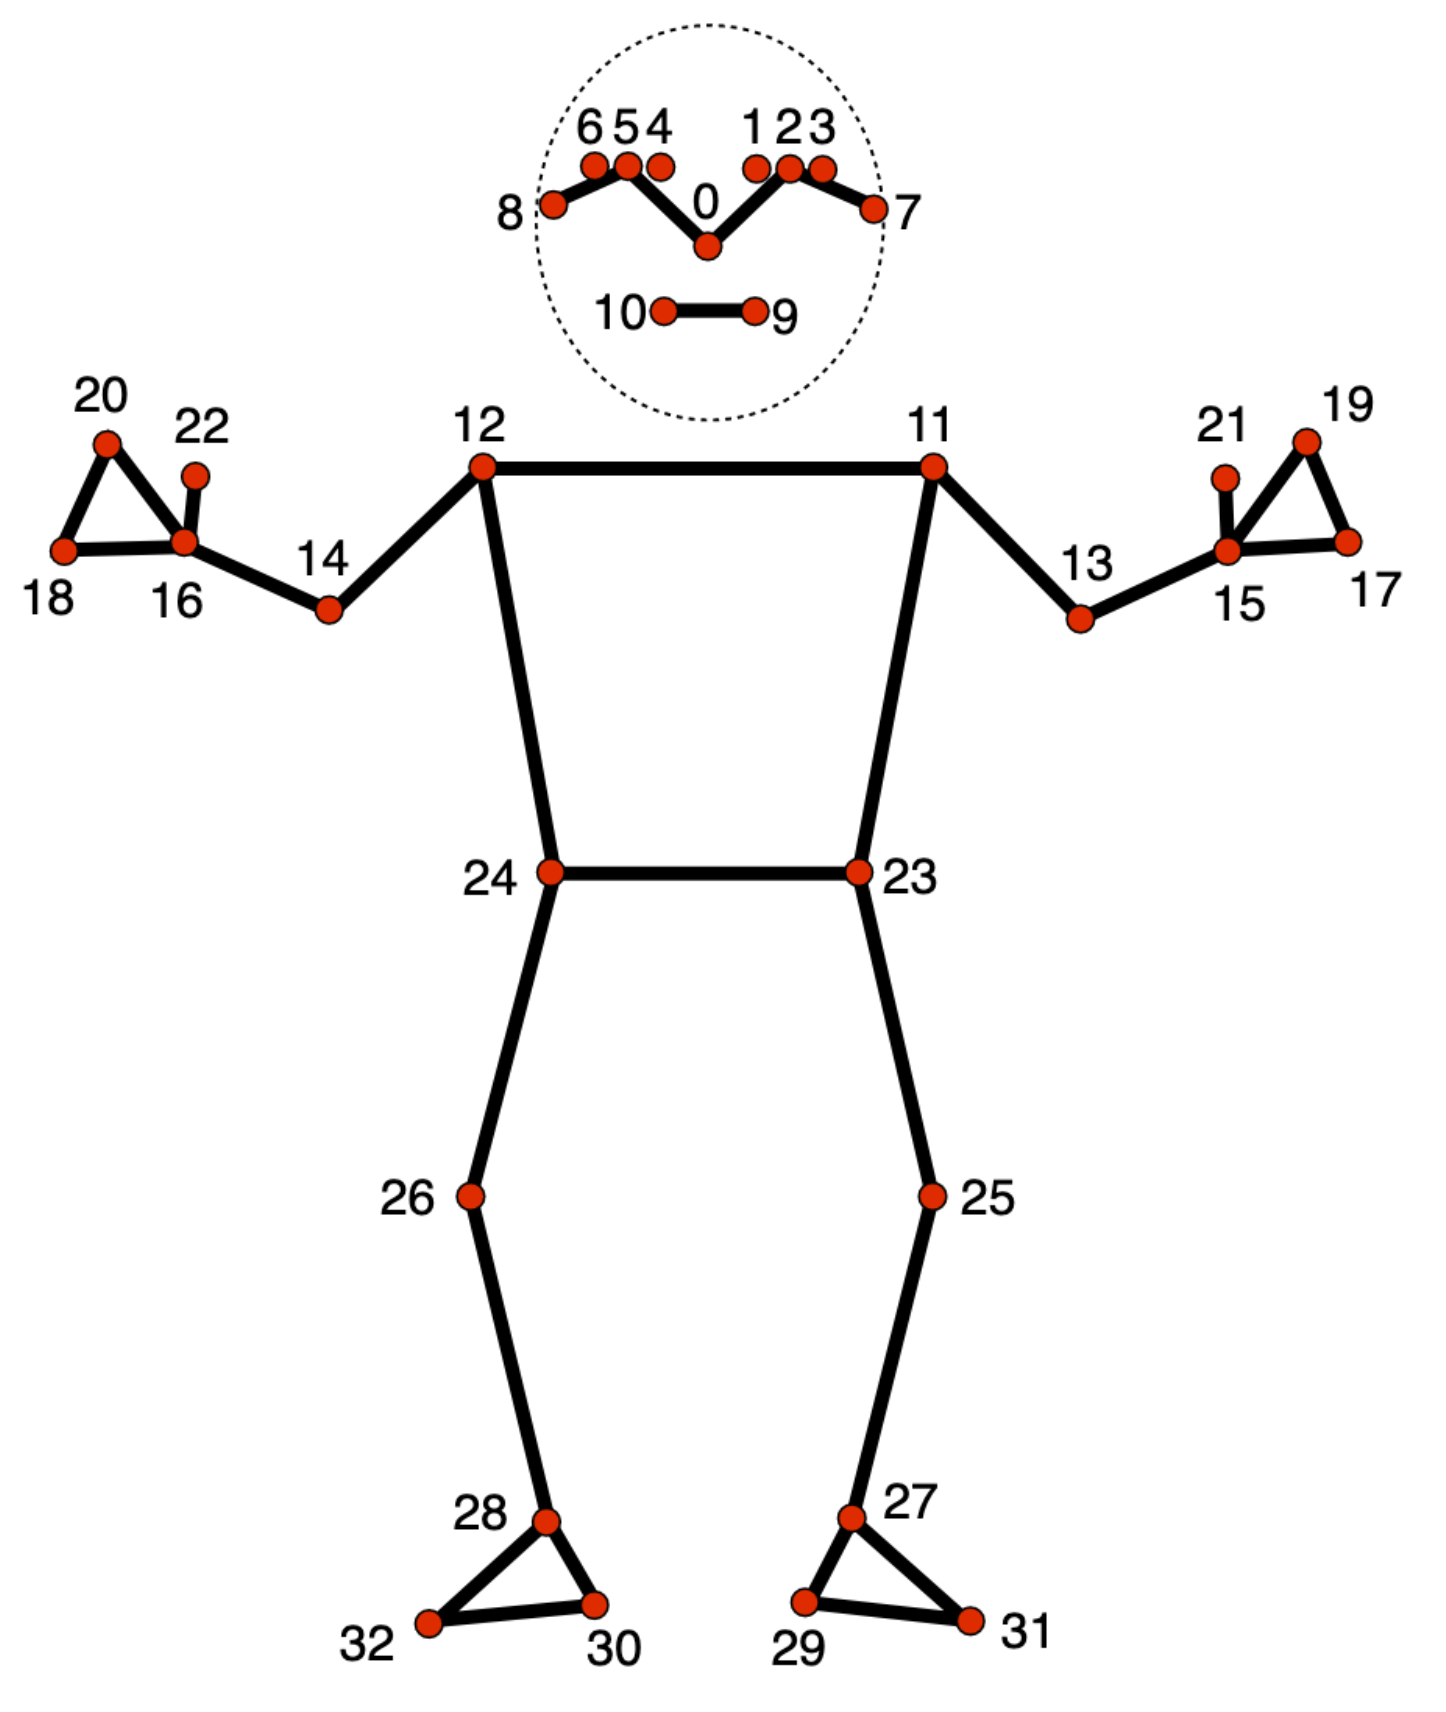
\includegraphics[scale=0.3]{figuras/eph/pose_landmarks.png}
  \legend{Fonte: \cite{mediapipe_pose_landmarker}}
	\label{fig:Pontos de referencia}
\end{figure}

\begin{itemize}
    \item[0] - nariz
    \item[1] - olho esquerdo (interno)
    \item[2] - olho esquerdo
    \item[3] - olho esquerdo (externo)
    \item[4] - olho direito (interno)
    \item[5] - olho direito
    \item[6] - olho direito (externo)
    \item[7] - orelha esquerda
    \item[8] - orelha direita
    \item[9] - boca (esquerda)
    \item[10] - boca (direita)
    \item[11] - ombro esquerdo
    \item[12] - ombro direito
    \item[13] - cotovelo esquerdo
    \item[14] - cotovelo direito
    \item[15] - pulso esquerdo
    \item[16] - pulso direito
    \item[17] - mindinho esquerdo
    \item[18] - mindinho direito
    \item[19] - indicador esquerdo
    \item[20] - indicador direito
    \item[21] - polegar esquerdo
    \item[22] - polegar direito
    \item[23] - quadril esquerdo
    \item[24] - quadril direito
    \item[25] - joelho esquerdo
    \item[26] - joelho direito
    \item[27] - tornozelo esquerdo
    \item[28] - tornozelo direito
    \item[29] - calcanhar esquerdo
    \item[30] - calcanhar direito
    \item[31] - dedo do pé esquerdo (indicador)
    \item[32] - dedo do pé direito (indicador)
\end{itemize}\label{lst:Pontos de referencia}

    \item GitHub: O GitHub é uma plataforma de hospedagem em nuvem, lançada em 10 de abril de 2008 originalmente desenvolvida pela GitHub Inc e atualmente mantida pela Microsoft Corporation. Essa plataforma faz uso do Git um sistemas de controle de versão que mantém um registro abrangente e detalhado de todas as alterações realizadas no código-base, permitindo um rastreamento preciso do histórico de mudanças e do progresso do desenvolvimento ao longo do tempo. Sua capacidade de facilitar a colaboração eficaz e de manter um histórico completo. Além de desempenhar um papel essencial na colaboração entre desenvolvedores, proporcionando um ambiente colaborativo para projetos compartilhados\cite{github}.

 \end{itemize}

Na busca por uma abordagem robusta e fundamentada para a analise quantitativa do uso de memoria, e tempo de execução, é imperativo descrever os materiais empregados na realização deste estudo e detalhar as características dos principais componentes relevantes para o desempenho durante o processamento da imagem, abaixo segue uma lista com as características:

\begin{itemize}

\item Notebook IdeaPad 3 82MF0004BR AMD Ryzen 7 5700U 15,6" 8GB 

\item Pocessador
\subitem CPU: AMD Ryzen 7 5700U with Radeon Graphics
\subitem Frequência de clock: 1400 MHz
\subitem Número de núcleos: 16
\subitem Thread(s) per núcleo: 2

\item Memória (RAM)
\subitem Tipo: DDR4
\subitem Capacidade: 8 GB
\subitem Frequência: 1600 Mhz

\item Placa de video
\subitem Nome: AMD Radeon RX Vega 8 Graphics
\subitem Driver em Uso: amdgpu
\subitem Capacidade de memória VRAM: 2.09 GB

\item Memoria (SSD)
\subitem Capacidade de armazenamento: 256 GB
\subitem Destinado a swap: 50 GB
\subitem Interface: M2
\subitem Protocolo: NVMe

\item Sistema operacional GNU/Linux
\subitem Distribuição: Linux Mint 20.2
\subitem Kernel: 5.15.0-76-generic
\subitem LSB Version: core-11.1.0ubuntu2-noarch:printing-11.1.0ubuntu2-noarch:security-11.1.0ubuntu2-noarch




\end{itemize}


\section[Método]{Método}\label{sec:Metodo}

No desenvolvimento deste trabalho, adotou-se uma abordagem que combina processo usual de elaboração de um trabalho acadêmico com a estruturação das etapas de um sistema de visão computacional, fazendo uso do pré processamento, segmentação, representação e descrição, reconhecimento e interpretação conforme documentado na literatura \cite{imagemMonocromatica}. Essa abordagem foi escolhida para o desenvolvimento de um artefato em nível de prova de conceito, envolvendo os conteúdos abordados, o que torna este trabalho uma contribuição original e prática para a área em questão. Portanto, foram realizadas as seguintes etapas:


 \begin{itemize}
   \item Realização de revisão da literatura abordando o uso de visão computacional associado ao treinamento físico.
   \item Escolha da linguagem de programação para desenvolvimento da ferramenta.
   \item Escolha das tecnologias para realização do processamento de imagem.
   \item Escolha da ferramenta utilizada para a detecção de pose humana.  
   \item Realização de revisão da literatura abordando a importância do movimento excêntrico para o ganho de força
   \item Criação de uma estrategia para detecção do movimento correto de barra fixa    
   \item Desenvolvimento de uma Ferramenta computacional para detecção da execução correta da barra fixa.
   \item Avaliação dos resultados.
   
 \end{itemize}
